\subsection{ErrorMint}
ErrorMint (\path{http://sourceforge.net/projects/errormint/}) is a java tool that can be used to analyze web server error messages and extract viable server informations like software name and version and operation system name and version.\\
ErrorMint consists of a main java class file (\code{controller.class}) and modules that can be selected in the command line prompt.
\begin{figure}[ht]
	\centering
	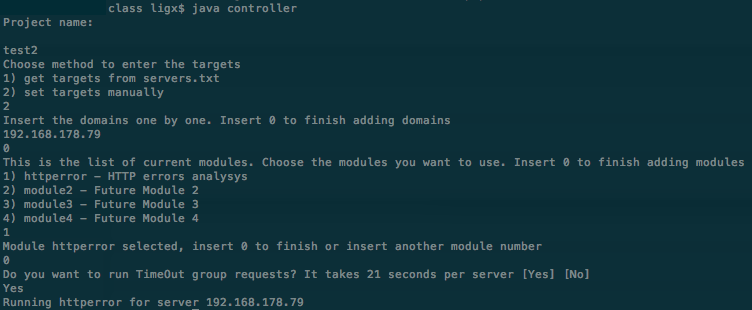
\includegraphics[width=.8\linewidth]{figures/OTG-ERR-001-1.png}
	\caption{ErrorMint in action}
	\label{fig:tool_sid_analysis}
\end{figure}
ErrorMint outputs a summary of the extracted information as well as html dumps of the error pages.
\begin{figure}[ht]
	\centering
	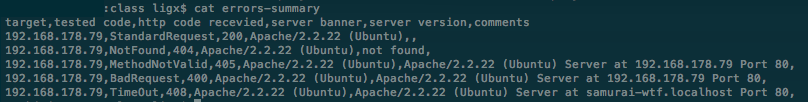
\includegraphics[width=.8\linewidth]{figures/OTG-ERR-001-2.png}
	\caption{ErrorMint in action}
	\label{fig:tool_error_mint}
\end{figure}
